\documentclass[11pt,a4paper]{article}
\usepackage[margin=1in]{geometry}
\usepackage{graphicx}
\usepackage{amsmath}
\usepackage[hidelinks]{hyperref}
\usepackage{authblk}
\usepackage{array}
\renewcommand{\arraystretch}{1.12}
\setlength{\parskip}{0.45em}
\setlength{\parindent}{0pt}
\title{Start-up of a randomized pilot trial of artificial intelligence feedback for NIH grant writing: outreach yield, data system readiness, and the failure of cold invitation}
\author\cite{r1,r2}{Ricardo Pietrobon\thanks{Corresponding author.}}
\author\cite{r1,r2}{Aline Machiavelli}
\author\cite{r1,r2}{Lucas Teixeira}
\author\cite{r1}{Luiza Paulsen Rodrigues}
\author\cite{r1}{Amit Agrey}
\author\cite{r1}{Lizzy Y. Nkeangnyi}
\author\cite{r1}{Giselle Zechia}
\author\cite{r1}{Victor Galv\~{a}o}
\author\cite{r3}{Paul Kuo}
\affil\cite{r1}{SporeData Inc, Durham, NC, USA}
\affil\cite{r2}{SporeData O\"{U}, Tallinn, Estonia}
\affil\cite{r3}{Department of Surgery, University of South Florida, Tampa, FL, USA}
\date{}
\begin{document}
\maketitle
\begin{abstract}
Artificial intelligence feedback is proposed as a scalable substitute for the scarce human review investigators need while drafting grant proposals, and no randomized trial has tested the claim. GRANT-AI is a parallel-group randomized pilot trial comparing large language model feedback with retrieval-augmented generation feedback, each combined with expert NIH reviewer comments, in investigators preparing NIH proposals. The trial received an exempt determination from the University of South Florida Institutional Review Board on 18 September 2025 and opened to recruitment with a target of 30 participants. We report the start-up record through 5 February 2026 from the study outreach tracker, the electronic data capture specification and its pre-trial test log, consent documents, and timestamped study files. Outreach covered 299 institution-department records at 152 distinct institutions. Ninety-four were searched for an eligible contact, 51 named contacts were identified, 23 introductory videoconferences took place, 28 invitations produced a recorded outcome, six investigators agreed to take part, two consented, and one submitted a proposal section and received feedback. Invitations issued after a videoconference produced agreement in six of seven cases; invitations issued without one produced agreement in none of 21 (Fisher exact p = $1.9 \times 10^{-5}$). The data capture system was specified at 66 fields across 13 forms and eight timepoints and passed 18 of 31 planned validation checks, yet six fields were ever populated. Readiness of the trial infrastructure ran far ahead of the recruitment that would have used it.
\end{abstract}
\noindent\textbf{Keywords:} pilot trials; recruitment; feasibility; artificial intelligence; grant writing; electronic data capture


\section{Introduction}

Investigators in clinical, translational and health services research compete for NIH funding against a success rate that has made the first independent award a career bottleneck rather than a milestone \cite{r1}. The remedy offered to them is feedback: a mentor who reads the Specific Aims, a colleague who has sat on a study section, an internal review panel. Mentoring of this kind is associated with research productivity and career advancement, although the evidence rests largely on cross-sectional and uncontrolled designs \cite{r2}. The supply is also fixed. Senior investigators able to critique a proposal are the same people writing their own, and the investigators who most need the critique are often those with the weakest access to it.

Structured programs have been built to widen that supply, and several report measured outcomes. The National Research Mentoring Network's Grant Writing Coaching Program reached 545 investigators at 187 institutions between June 2015 and March 2019 and tracked their subsequent submissions and awards \cite{r3}. A presubmission mock review program for postdoctoral fellows and early-career faculty enrolled 212 applicants between 2014 and 2021; of 194 applications with outcome data, 71 were funded, a 37 percent success rate \cite{r4}. An internal presubmission review program at the University of California, San Francisco reported that 44 percent of proposals reviewed over a 12-month period were subsequently funded, above the NIH success rate for the same period \cite{r5}. A grant writing course for early-career faculty at the University of California, San Diego \cite{r6} and a set of strategies delivered across Mountain West institutions \cite{r7} report similar activity. All of them consume senior reviewer time, which is the constraint they were meant to relieve.

Large language models are the obvious candidate replacement, and the evidence base for them in medicine has grown quickly without converging on much. A systematic review of 519 studies of healthcare applications found that 5 percent used real patient care data and that evaluation was dominated by accuracy on question answering rather than effects on any human outcome \cite{r8}. Retrieval-augmented generation, which grounds model output in a curated document set, has been reviewed across healthcare applications \cite{r9} and implemented as a hepatology chat interface grounded on 30 society guidance documents, which answered all 10 questions of a published knowledge assessment correctly \cite{r10}. Applied to review rather than to care, the results are mixed and the comparisons are small. One feasibility study compared ChatGPT's critique against human reviews of a single published case report \cite{r11}, transformer models fine-tuned on three years of reviewer comments at the Journal of Neurosurgery were used to predict acceptance against rejection \cite{r12}, and a comparison at the American Journal of Sports Medicine concluded that the model could support editorial triage but not replace reviewers \cite{r13}. Two blinded randomized non-inferiority studies found model-written plain-language summaries \cite{r14} and introduction sections \cite{r15} rated comparably to human-written text, which is a claim about prose rather than about critique.

Grant writing has not been tested this way. Reviews of ChatGPT in academic writing identify the gap and do not fill it \cite{r16}, and the one grant-specific tool we found, GrantCheck, is reported as a development study aligning proposal language to policy requirements with no trial of its effect on the investigator \cite{r17}. Editorial and integrity guidance has nonetheless arrived first, telling authors how to disclose model assistance \cite{r18} and surveying editors on how to handle it \cite{r19}. The field is accumulating policy on an intervention nobody has randomized.

We designed GRANT-AI to randomize it. Before effectiveness, a pilot has to establish that the trial can be run at all, which is the purpose the CONSORT extension to pilot and feasibility trials assigns to this stage \cite{r20,r21} and the reason progression criteria are set in advance \cite{r22}. Reporting below follows that extension, with the CONSORT 2025 statement \cite{r23} as the parent guideline, to the extent the trial reached. Recruitment is the usual place where that question is answered badly. The Cochrane review of strategies to improve recruitment to randomized trials found only 3 of 72 comparisons supported by high-certainty evidence, and its 2026 update draws on studies embedded within host trials \cite{r24,r25}. Every one of those comparisons concerns approaching patients. GRANT-AI recruits investigators: busy, senior, approached through institutional hierarchies, and asked to put an unsubmitted grant proposal into someone else's platform. We could find no trial methodology evidence addressed to that population.

This paper reports what start-up produced. It is not the trial result, and the trial has not reached the sample at which its randomized comparison becomes interpretable. It is the record of how 299 institutional approaches converted into two consented participants over seven months, what the conversion depended on, and how much trial infrastructure was built and validated for data that never arrived. Reporting that record is the alternative to adding one more unfinished trial to the stock of research waste \cite{r26}.

\section{Methods}

\subsection{Trial design and oversight}

GRANT-AI is a parallel-group, mixed-methods randomized pilot trial. Participants are randomized 1:1 to receive structured feedback on NIH proposal sections from a large language model aligned to NIH review criteria, or from a retrieval-augmented generation system drawing on a curated corpus of funded proposals, reviewer summary statements and institutional guidance. Both arms also receive written critique from a single expert reviewer (RP) with more than 25 years of experience reviewing NIH clinical research applications. Both platforms carry behavioral engagement features, including progress tracking and peer comparison, of the kind tested in randomized gamification trials outside this domain \cite{r27}. Participants submit Specific Aims, Significance/Innovation and Approach within a 90-day window, revise against feedback, and are offered a semi-structured interview afterwards. Eligibility requires an investigator at a United States clinical department who is actively preparing an NIH proposal involving human data. The planned sample was 30.

The protocol received an exempt determination (Exempt category 3) from the University of South Florida Institutional Review Board on 18 September 2025 under IRB ID STUDY008974, with Dr Paul Kuo as principal investigator. The trial was not prospectively registered in a public registry, which we report as a protocol deviation from ICMJE expectations rather than defend.

\subsection{Recruitment procedure}

Recruitment proceeded by institution rather than by advertisement. Members of the study team compiled a list of United States medical schools and academic medical centers, then searched each institution for a named individual in a target department who was positioned to identify eligible investigators, typically a vice chair for research, a research director or a division chief. Where a name and address were found, the team sent an introductory email offering a videoconference. Where a videoconference took place, the study was described and the contact was asked either to participate or to refer eligible colleagues. Two departmental strata were worked in sequence: Internal Medicine first, from 2 July 2025, and Surgery afterwards. A third block of institutions was listed without a departmental assignment and had not been worked at the census date.

\subsection{Data sources and census date}

This analysis uses five sources held in the study's shared drive: the recruitment tracker, a spreadsheet with one row per institution-department record and columns for search status, named contact, email address, completed videoconference, and invitation outcome; the case report form specification, listing every planned variable with its type, parent form and timepoint; the pre-trial testing checklist for the electronic data capture system; the consent documents on file; and the creation and modification timestamps of all 56 study files, which provide the start-up chronology. We took 5 February 2026 as the census date, the last date on which the recruitment tracker was modified. All counts are as of that date. No participant is identified; institutional and contact names were used only to link records across sources and are not reported.

\subsection{Outcomes}

The feasibility outcomes are those specified in the protocol for recruitment and engagement, evaluated at the stage the trial had reached. They are: the number of institutions approached and the proportion yielding a named contact; the proportion of named contacts yielding a completed videoconference, an invitation outcome, and an agreement to participate; the number consenting; the number submitting at least one proposal section and receiving at least one feedback iteration; and elapsed time from first outreach to first consent. We added one outcome not in the protocol, after inspecting the tracker: agreement to participate conditional on whether an introductory videoconference preceded the invitation. Readiness outcomes are the size and structure of the data capture specification, the proportion of planned pre-trial validation checks executed, and the proportion of specified fields ever populated.

\subsection{Statistical analysis}

Analysis is descriptive. Proportions are reported with the stage denominators stated in each table. The association between a prior videoconference and agreement to participate was tested with Fisher's exact test among the 28 contacts with a recorded invitation outcome, and agreement proportions are reported with Jeffreys 95 percent intervals, which behave sensibly at a zero numerator. No modelling was attempted; with two consented participants there is nothing to adjust. Analyses used Python 3.11.15 with pandas 2.3.3 and SciPy 1.17.1.

\section{Results}

\subsection{Outreach volume and contact identification}

The tracker held 299 institution-department records covering 152 distinct institutions (Table 1; the full cross-tabulation by stratum and invitation outcome is Table A.3). Work was uneven across strata by design, because the strata were worked in sequence. Every one of the 65 Internal Medicine records was searched for a contact and 44 yielded a named individual, a hit rate of 67.7 percent. Of the 135 Surgery records, 23 were searched and seven yielded a name. The 99 unassigned records produced six searches and no names. Across all strata, searching an institution identified a usable contact in 51 of 94 cases (54.3 percent), and in the fully worked Internal Medicine stratum in 44 of 65 (67.7 percent), so the hit rate was adequate. What held the funnel back was how few institutions had been searched at all: 94 of 299 records, or 31.4 percent.

\subsection{Progression through the funnel}

Table 2 and Figure 1 give the funnel. Of 51 named contacts, 49 had an email address recorded and 23 completed an introductory videoconference. Twenty-eight invitations had a recorded outcome, six of which were agreements to participate and 21 of which were recorded as no response; one contact offered to consider referring colleagues. Two informed consent forms are on file, dated 7 January 2026 and 14 January 2026. One participant submitted a Specific Aims draft on 12 January 2026 and received a 772-word structured critique organized into three numbered domains on 22 January 2026, ten days later. No participant completed a second section, and no randomization record exists for either consented participant.

Elapsed time from the first tracker entry on 2 July 2025 to the first consent on 7 January 2026 was 189 days. From the IRB exempt determination to first consent was 111 days. Measured against the planned sample of 30, enrollment at the census date was 6.7 percent.

The one participant whose institution could be traced through the tracker was enrolled from an institution where a departmental contact had already agreed to take part, and sits in a department (occupational therapy education) outside the Internal Medicine stratum that had been worked and outside the clinical departments named in the eligibility criteria. The second consent form carries a typed name and date with the signature line blank; the first is a signed scan. Neither carries the countersignature of the person obtaining consent.

\subsection{Invitations with and without a prior videoconference}

Among the 28 contacts with a recorded invitation outcome, every agreement followed a videoconference (Table 3). Six of seven invitations issued after a videoconference produced agreement (85.7 percent, 95 percent CI 49.9 to 98.4) and the seventh produced an offer to refer colleagues. None of the 21 invitations issued without a prior videoconference produced any response at all (0 percent, 95 percent CI 0 to 11.1). Fisher's exact test gives p = $1.9 \times 10^{-5}$. The 16 contacts who completed a videoconference but have no invitation outcome recorded were still open at the census date and are excluded from this comparison.

\subsection{Data system readiness}

The case report form specification defined 66 variables across 13 forms and eight study timepoints, from enrollment through a six-month post-submission follow-up (Table A.1, with the field-type breakdown in Table A.4). Field types were binary (15), text (13, including one list field), categorical (11), numeric (16 across three variants), date (8), ordinal (2) and checkbox (1). Pre-trial validation was planned as 31 checks in nine categories (Table 4; the checks verbatim, with the testers' comments, are Table A.2). Eighteen were executed and recorded as passed, including range limits, required-field enforcement, branching logic, navigation between instruments, form completion status, user role permissions and the three reporting and dashboard checks. Ten were deferred or marked not applicable, among them both external tool and API checks and the calculated-field check. Three were unresolved at census: two of the three user acceptance testing items, which had no entry, and one workflow item carrying an open question about whether the eight declared timepoints were distinct study events.

Against that build, six of 66 specified fields were ever populated, all of them on the enrollment form of a single participant: institution, department, career stage, gender, race or ethnicity, and highest degree. Twelve of the 13 forms were never opened. Intervention content was also in place ahead of demand: four worked feedback examples totalling 6,911 words, covering Specific Aims, Significance, Innovation and Approach, were produced on 10 November 2025, two months before the first participant draft arrived. Figure 2 places every build milestone against the recruitment it was built to serve; the dated milestones are listed in Table A.5.

\section{Discussion}

A trial designed to randomize 30 investigators to two forms of artificial intelligence feedback approached 152 institutions over seven months, obtained six verbal agreements, consented two, and delivered one feedback iteration to one person. The infrastructure built to receive those data was specified at 66 fields, tested against 31 checks, and used for six values. The start-up record contains one finding with a defensible effect size, one with a clear shape and a small denominator, and one that is about where effort went.

The first is that the invitation did not work without a conversation. Every one of the six agreements came after a videoconference, and none of the 21 invitations sent without one drew any reply (Table 3). An odds ratio is not estimable with a zero cell. The comparison is 6 of 7 against 0 of 21, with Fisher exact p = $1.9 \times 10^{-5}$. The direction is consistent with what is known about reaching physicians through written approaches: mailed physician questionnaires average 61 percent response, falling to 52 percent for samples above 1,000 \cite{r28}; a web survey of 904 specialists in one Canadian city returned 35.0 percent \cite{r29}; and a randomized experiment at the American Board of Internal Medicine moved response from 18.2 percent with email reminders alone to 43.1 percent with postcards, paper surveys and a \$1 incentive \cite{r30}. Across 68 American Academy of Pediatrics surveys from 2000 to 2019, mean response was 56.2 percent and declined year on year \cite{r31}. Our result is stronger than those because the request is heavier than a survey, and the practical reading is that for this population the videoconference is not a courtesy preceding the ask, it is the recruitment intervention. The cost follows from that. Twenty-three videoconferences across seven months is a rate that cannot produce 30 participants in any reasonable horizon, which is the arithmetic the trial failed to do before it opened.

The second is that most of the loss happens before any investigator is approached. Of 299 institution-department records, 94 were searched and 51 produced a named contact (Table 1 and Table 2). The search step, not the persuasion step, is where 205 records sat untouched. When a search was done it yielded a name in 51 of 94 cases (54.3 percent), rising to 67.7 percent in the one stratum worked to completion, so the problem is throughput rather than yield. This is an inversion of the usual recruitment picture, where the sampling frame is a clinic list and the attrition sits at approach and consent; in 73 UK publicly funded trials, 55 percent reached their target sample and 78 percent reached 80 percent of it, with the shortfall arising downstream of a defined frame \cite{r32,r33}. The recruitment literature here is built on patient populations \cite{r24,r34,r35} and on the behavior of clinicians recruiting their patients \cite{r36}, and neither maps onto an investigator-participant reached through a departmental hierarchy. The one enrollment we could trace arrived by referral from a contact at an institution that had already agreed, and came from a department outside both the worked stratum and the stated eligibility criteria. A single case is no evidence of a mechanism. It does point where the next design should look: at the agreed contact as a recruiting node rather than as a participant, which is closer to how mentoring and faculty development interventions actually propagate \cite{r37}.

The third is that readiness and recruitment were sequenced in the wrong order. Between May and December 2025 the team specified 66 fields, built 13 forms across eight timepoints, ran 18 validation checks, drafted consent and FAQ materials, recorded a study video, and produced four worked feedback examples totalling 6,911 words. Over the same period, 23 videoconferences took place. The validation work itself was sound as far as it went, and REDCap-based studies that skip it pay for it later \cite{r38,r39,r40,r41}; what was wrong was its position in the queue. Thirteen of the 31 checks remain deferred or unresolved, including both API checks and two of the three user acceptance tests, and user acceptance testing is precisely the check that needs participants. Progression criteria would have caught this. The CONSORT pilot extension asks for them \cite{r20} and recommendations exist for setting them \cite{r22}. A methodological review of 160 external pilot publications that did report progression criteria found 133 (83 percent) expressed them as fixed thresholds \cite{r42}, and a meta-research study of surgical pilot and feasibility trials found reporting against the CONSORT extension incomplete in both 2011 and 2021 \cite{r43}. GRANT-AI set a sample target and no recruitment checkpoint, so there was no date at which a rate of 23 conversations per seven months triggered a decision.

Several limitations bound these conclusions. The tracker is an operational working document, not a prospectively specified data collection instrument: a blank cell can mean not done, done and not recorded, or not applicable, and we have treated blanks as not done, which biases every denominator towards pessimism. The videoconference comparison is observational and confounded by selection in the obvious direction, since contacts who accept a meeting are more willing before the invitation is issued; the honest claim is that no cold invitation succeeded, not that the meeting caused the agreement. Sixteen contacts with completed videoconferences had no recorded outcome and are excluded from Table 3, and if they resolve as refusals the agreement proportion after a meeting falls from 85.7 percent to 26.1 percent. Timeline dates are file creation timestamps rather than logged events, so they bound rather than measure when work happened. No outcome of the randomized comparison is reported here because none exists: no participant was randomized, and nothing in this paper speaks to whether retrieval-augmented feedback outperforms a general language model. Attrition after enrollment is likewise unassessed at this depth, although the pattern of a single engagement followed by silence is familiar from digital intervention cohorts \cite{r44}.

What we would do differently is specific. Recruitment of investigator-participants should be costed in videoconferences rather than in emails, with a target rate set in advance and a progression criterion that stops the trial if the rate is not met by a stated date. The unit of recruitment should be the agreed departmental contact, with an explicit referral mechanism and a count of referrals produced per contact, since that is the only path by which our one engaged participant arrived. Data system build should be staged against enrollment rather than completed ahead of it, with user acceptance testing scheduled for the first consented participants instead of planned and left undone. A future version of this trial should also be registered before the first approach. Whether artificial intelligence feedback improves NIH proposals remains open, and will stay open until a trial of it reaches the investigators it is meant to help.

\section*{Declarations}

Ethics approval. The GRANT-AI protocol received an exempt determination (Exempt category 3) from the University of South Florida Institutional Review Board on 18 September 2025, IRB ID STUDY008974, with Dr Paul Kuo as principal investigator. All enrolled participants provided written informed consent. No individual participant is identifiable in this report.

Trial registration. The trial was not prospectively registered in a public trial registry. We report this as a deviation from ICMJE expectations.

Funding. This work was supported by SporeData Inc (Durham, NC, USA). No external sponsor had any role in study design, data collection, analysis, or the decision to submit.

Supplementary material. A supplementary appendix contains Tables A.1 to A.6, a sensitivity analysis for the 16 unresolved contacts (A.7), the basis for the novelty claim (A.8) and a reproducibility statement (A.9).

Declaration of competing interest. RP, AM, LT, LPR, AA, LYN, GZ and VG are affiliated with SporeData Inc, which developed the GRANT-AI feedback platform under evaluation. RP served as the expert NIH reviewer within the trial and is an author of this report; he had no role in the independent blinded outcome assessment, which the trial did not reach by the census date. PK is the principal investigator of record and reports no competing interest.

Data and code availability. The de-identified recruitment tracker, the case report form specification, the pre-trial testing checklist, the study timeline and the analysis code that regenerates every number, table and figure in this manuscript are archived at https://github.com/ricardopietrobon/grant-ai. Running analysis/reproduce.py re-derives 34 published values and fails if any does not match; analysis/test\_published\_values.py checks 24 named manuscript claims. Institution identity is replaced by a salted SHA-256 surrogate and personal names and addresses are removed; the unredacted tracker is available from the corresponding author under a data use agreement. Limits on what the archive can reproduce are stated in Appendix A.9.

CRediT authorship contribution statement. Ricardo Pietrobon: Conceptualization, Methodology, Formal analysis, Investigation, Writing - original draft, Supervision. Aline Machiavelli: Methodology, Data curation, Investigation, Writing - review and editing. Lucas Teixeira: Software, Data curation, Writing - review and editing. Luiza Paulsen Rodrigues: Investigation, Data curation. Amit Agrey: Investigation, Project administration. Lizzy Y. Nkeangnyi: Investigation, Project administration. Giselle Zechia: Investigation, Data curation. Victor Galvao: Software, Validation. Paul Kuo: Conceptualization, Supervision, Writing - review and editing.

Declaration of generative AI and AI-assisted technologies in the writing process. During the preparation of this work the authors used a large language model to draft and edit sections of the manuscript and to tabulate the study operational records. The authors reviewed and edited the content as needed and take full responsibility for the content of the published article. The feedback systems evaluated inside the trial are the object of study and are described in the Methods.


\begin{figure}[htbp]\centering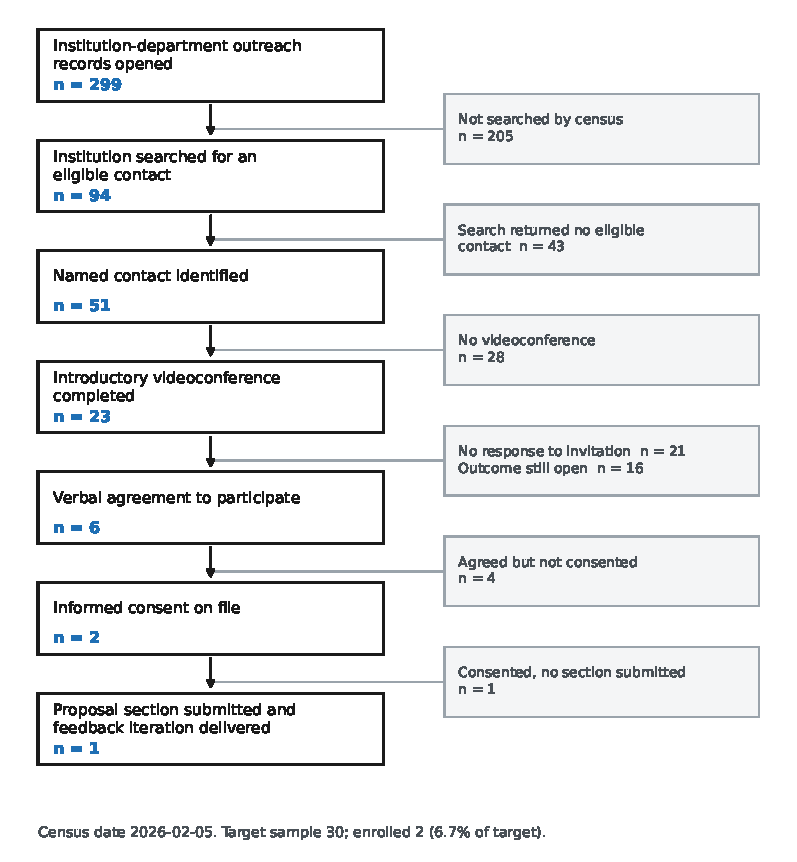
\includegraphics[width=0.78\textwidth]{figure_1_recruitment_flow.pdf}
\caption{Recruitment flow from institutional outreach to feedback delivery, GRANT-AI pilot trial, 2 July 2025 to the census date of 5 February 2026. Boxes on the left give the number of institution-department records reaching each stage; boxes on the right give the losses between stages. The invitation stage does not nest cleanly within the videoconference stage: 21 of the 28 recorded invitation outcomes belong to contacts who had no videoconference, and 16 contacts who did have one had no outcome recorded at census.}\label{fig:flow}\end{figure}
\begin{figure}[htbp]\centering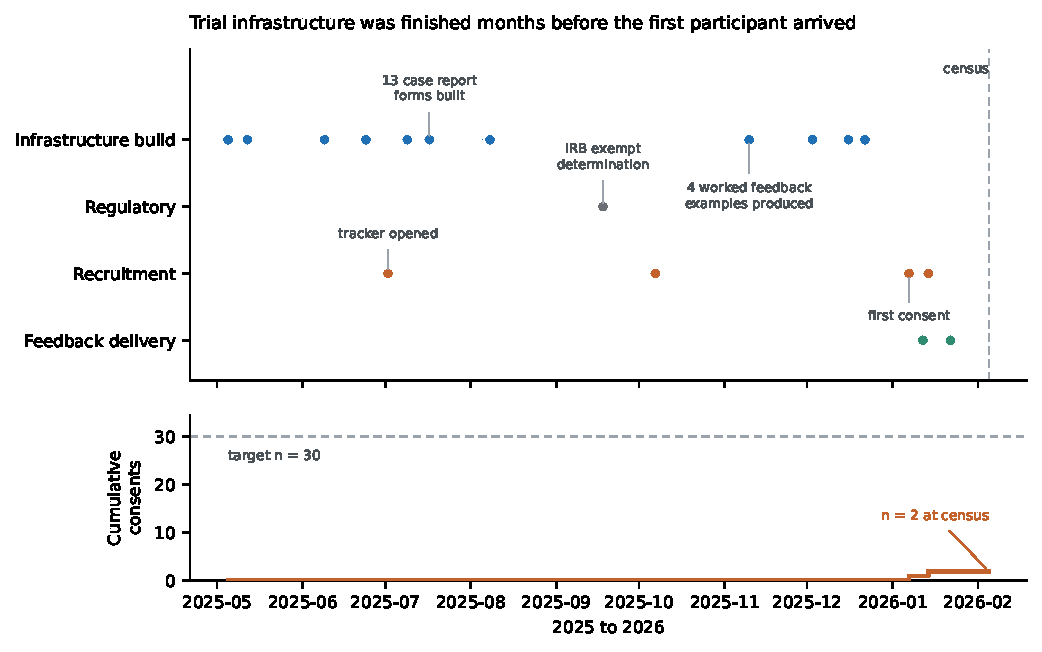
\includegraphics[width=\textwidth]{figure_2_timeline.pdf}
\caption{Study milestones by category against cumulative enrollment. Upper panel: each point is a dated study file or regulatory event, assigned to infrastructure build, regulatory, recruitment or feedback delivery. Lower panel: cumulative informed consents against the planned sample of 30. The thirteen case report forms and the four worked feedback examples were complete in July and November 2025 respectively; the first consent arrived on 7 January 2026, 189 days after the recruitment tracker was opened.}\label{fig:timeline}\end{figure}


\begin{table}[htbp]
\centering
\small
\caption{Outreach volume and contact identification by departmental stratum, GRANT-AI pilot trial, 2 July 2025 to 5 February 2026. Institutions are counted within stratum; the 152 distinct institutions in the total row are fewer than the stratum sum because institutions appear in more than one stratum.}
\label{tab:outreach}
\begin{tabular}{lrrrrr}
\hline
\textbf{Departmental stratum} & \textbf{Outreach records} & \textbf{Distinct institutions} & \textbf{Institutions searched for a contact} & \textbf{Named contacts identified} & \textbf{Contact email addresses obtained} \\
\hline
Internal Medicine & 65 & 51 & 65 & 44 & 43 \\
Surgery & 135 & 134 & 23 & 7 & 6 \\
Unassigned & 99 & 99 & 6 & 0 & 0 \\
Total & 299 & 152 & 94 & 51 & 49 \\
\hline
\end{tabular}
\end{table}


\begin{table}[htbp]
\centering
\small
\caption{Progression through the recruitment funnel to the census date of 5 February 2026. The invitation row does not nest within the videoconference row: 21 of the 28 recorded invitations were issued without a preceding videoconference.}
\label{tab:funnel}
\begin{tabular}{lrr}
\hline
\textbf{Stage} & \textbf{n} & \textbf{\% of 299 outreach records} \\
\hline
Outreach records opened & 299 & 100.0 \\
Institution searched for an eligible contact & 94 & 31.4 \\
Named contact identified & 51 & 17.1 \\
Contact email address obtained & 49 & 16.4 \\
Introductory videoconference completed & 23 & 7.7 \\
Study invitation with a recorded outcome & 28 & 9.4 \\
Verbal agreement to participate & 6 & 2.0 \\
Informed consent form on file & 2 & 0.7 \\
At least one proposal section submitted & 1 & 0.3 \\
At least one feedback iteration delivered & 1 & 0.3 \\
\hline
\end{tabular}
\end{table}


\begin{table}[htbp]
\centering
\small
\caption{Invitation outcome by whether an introductory videoconference preceded the invitation, among the 28 contacts with a recorded outcome. Intervals are Jeffreys 95 percent intervals. Fisher exact p = 1.9 x 10\textasciicircum{}-5. Sixteen contacts who completed a videoconference had no recorded invitation outcome and are excluded.}
\label{tab:invite}
\begin{tabular}{lrrrrr}
\hline
\textbf{Introductory videoconference before invitation} & \textbf{Invitations} & \textbf{Agreed to participate} & \textbf{No response} & \textbf{Other response} & \textbf{Agreement, \% (95\% CI)} \\
\hline
Yes & 7 & 6 & 0 & 1 & 85.7 (49.9-98.4) \\
No & 21 & 0 & 21 & 0 & 0.0 (0.0-11.1) \\
Total & 28 & 6 & 21 & 1 & 21.4 \\
\hline
\end{tabular}
\end{table}


\begin{table}[htbp]
\centering
\small
\caption{Pre-trial validation of the electronic data capture system by test category. Items marked deferred or not applicable carried an explicit dash in the testing log; unresolved items had no entry.}
\label{tab:validation}
\begin{tabular}{lrrrr}
\hline
\textbf{Test category} & \textbf{Items} & \textbf{Executed} & \textbf{Deferred or not applicable} & \textbf{Unresolved at census} \\
\hline
1. Field Validation & 6 & 4 & 2 & 0 \\
2. Input Type Consistency & 3 & 2 & 1 & 0 \\
3. Workflow Simulation & 4 & 3 & 0 & 1 \\
4. Import/Export Tests & 3 & 2 & 1 & 0 \\
5. Quality Checks & 4 & 2 & 2 & 0 \\
6. External Tools / APIs & 2 & 0 & 2 & 0 \\
7. Reports / Dashboards & 3 & 3 & 0 & 0 \\
8. UAT Feedback & 3 & 0 & 1 & 2 \\
9. Extra Tests & 3 & 2 & 1 & 0 \\
Total & 31 & 18 & 10 & 3 \\
\hline
\end{tabular}
\end{table}


\begin{thebibliography}{99}
\small

\bibitem{r1} Ley TJ, Rosenberg LE. The physician-scientist career pipeline in 2005: build it, and they will come. JAMA. 2005;294(11):1343-1351. doi:10.1001/jama.294.11.1343.

\bibitem{r2} Sambunjak D, Straus SE, Marusić A. Mentoring in academic medicine: a systematic review. JAMA. 2006;296(9):1103-1115. doi:10.1001/jama.296.9.1103.

\bibitem{r3} Weber-Main AM, McGee R, Eide Boman K, et al. Grant application outcomes for biomedical researchers who participated in the National Research Mentoring Network's Grant Writing Coaching Programs. PLoS One. 2020;15(11):e0241851. doi:10.1371/journal.pone.0241851.

\bibitem{r4} Castillo-Mancilla JR, Erlandson KM, Hecker ER, et al. Outcomes of a Career Development Award (Pre-K) Mock Review Program for Postdoctoral Fellows and Early-Career Faculty. Acad Med. 2023;98(11):1313-1318. doi:10.1097/ACM.0000000000005293.

\bibitem{r5} Johnson MO, Neilands TB, Kegeles SM, Gaffney S, Lightfoot MA. The Architecture of an Internal, Scientific, Presubmission Review Program Designed to Increase the Impact and Success of Grant Proposals and Manuscripts. Acad Med. 2020;95(2):200-206. doi:10.1097/ACM.0000000000003008.

\bibitem{r6} LaCroix AZ, Fettes D, Serin Y, et al. Building strong grant writers in academic medicine: outcomes of early-career faculty enrolled in the University of California San Diego Health Sciences Grant Writing Course. Acad Med. 2026;101(1):34-42. doi:10.1093/acamed/wvaf031.

\bibitem{r7} Dagda RK, Myaskovsky L, Sood A, et al. Evidence-based strategies for delivering grant writing skills to clinical and translational science faculty in the Mountain West. J Clin Transl Sci. 2025;9(1):e268. doi:10.1017/cts.2025.10198.

\bibitem{r8} Bedi S, Liu Y, Orr-Ewing L, et al. Testing and Evaluation of Health Care Applications of Large Language Models: A Systematic Review. JAMA. 2025;333(4):319-328. doi:10.1001/jama.2024.21700.

\bibitem{r9} Amugongo LM, Mascheroni P, Brooks S, Doering S, Seidel J. Retrieval augmented generation for large language models in healthcare: A systematic review. PLOS Digit Health. 2025;4(6):e0000877. doi:10.1371/journal.pdig.0000877.

\bibitem{r10} Ge J, Sun S, Owens J, et al. Development of a liver disease-specific large language model chat interface using retrieval-augmented generation. Hepatology. 2024;80(5):1158-1168. doi:10.1097/HEP.0000000000000834.

\bibitem{r11} Biswas S, Dobaria D, Cohen HL. ChatGPT and the Future of Journal Reviews: A Feasibility Study. Yale J Biol Med. 2023;96(3):415-420. doi:10.59249/SKDH9286.

\bibitem{r12} Hopkins BS, Shah I, Dallas J, et al. Application of large language and artificial intelligence modeling in the prediction of peer-review outcomes. J Neurosurg. 2025;144(3):720-728. doi:10.3171/2025.8.JNS242667.

\bibitem{r13} Patel R, Shultz C, Ollivier M, Wascher DC. Artificial Intelligence Cannot Replace Peer Reviewers but May Help Editors Triage: A Comparative Analysis of a Large Language Model and Human Reviewer Recommendations at the American Journal of Sports Medicine. Am J Sports Med. 2026;54(11):2800-2807. doi:10.1177/03635465261463006.

\bibitem{r14} Ágústsdóttir DH, Rosenberg J, Baker JJ. ChatGPT-4o Compared With Human Researchers in Writing Plain-Language Summaries for Cochrane Reviews: A Blinded, Randomized Non-Inferiority Controlled Trial. Cochrane Evid Synth Methods. 2025;3(4):e70037. doi:10.1002/cesm.70037.

\bibitem{r15} Sikander B, Baker JJ, Deveci CD, Lund L, Rosenberg J. ChatGPT-4 and Human Researchers Are Equal in Writing Scientific Introduction Sections: A Blinded, Randomized, Non-inferiority Controlled Study. Cureus. 2023;15(11):e49019. doi:10.7759/cureus.49019.

\bibitem{r16} Liu Y, Kong W, Merve K. ChatGPT applications in academic writing: a review of potential, limitations, and ethical challenges. Arq Bras Oftalmol. 2025;88(3). doi:10.5935/0004-2749.2024-0269.

\bibitem{r17} Shi Q, Oztekin A, Matthew G, et al. GrantCheck-an AI Solution for Guiding Grant Language to New Policy Requirements: Development Study. JMIR Form Res. 2025;9:e79038. doi:10.2196/79038.

\bibitem{r18} Leung TI, de Azevedo Cardoso T, Mavragani A, Eysenbach G. Best Practices for Using AI Tools as an Author, Peer Reviewer, or Editor. J Med Internet Res. 2023;25:e51584. doi:10.2196/51584.

\bibitem{r19} Biondi-Zoccai G, Lauretti A, Agewall S, et al. Perspectives on Artificial Intelligence in Medical Publishing: A Survey of Medical Journal Editors. J Cardiovasc Pharmacol. 2025;86(4):374-383. doi:10.1097/FJC.0000000000001738.

\bibitem{r20} Eldridge SM, Chan CL, Campbell MJ, et al. CONSORT 2010 statement: extension to randomised pilot and feasibility trials. BMJ. 2016;355:i5239. doi:10.1136/bmj.i5239.

\bibitem{r21} Eldridge SM, Lancaster GA, Campbell MJ, et al. Defining Feasibility and Pilot Studies in Preparation for Randomised Controlled Trials: Development of a Conceptual Framework. PLoS One. 2016;11(3):e0150205. doi:10.1371/journal.pone.0150205.

\bibitem{r22} Mellor K, Albury C, Dutton SJ, Eldridge S, Hopewell S. Recommendations for progression criteria during external randomised pilot trial design, conduct, analysis and reporting. Pilot Feasibility Stud. 2023;9(1):59. doi:10.1186/s40814-023-01291-5.

\bibitem{r23} Hopewell S, Chan AW, Collins GS, et al. CONSORT 2025 statement: updated guideline for reporting randomised trials. BMJ. 2025;389:e081123. doi:10.1136/bmj-2024-081123.

\bibitem{r24} Treweek S, Pitkethly M, Cook J, et al. Strategies to improve recruitment to randomised trials. Cochrane Database Syst Rev. 2018;2(2):MR000013. doi:10.1002/14651858.MR000013.pub6.

\bibitem{r25} Parker A, Mongelli G, Piccolo-Lawrance C, et al. Strategies to improve recruitment to randomised trials. Cochrane Database Syst Rev. 2026;9(9):MR000013. doi:10.1002/14651858.MR000013.pub7.

\bibitem{r26} Chalmers I, Glasziou P. Avoidable waste in the production and reporting of research evidence. Lancet. 2009;374(9683):86-89. doi:10.1016/S0140-6736(09)60329-9.

\bibitem{r27} Patel MS, Bachireddy C, Small DS, et al. Effect of Goal-Setting Approaches Within a Gamification Intervention to Increase Physical Activity Among Economically Disadvantaged Adults at Elevated Risk for Major Adverse Cardiovascular Events: The ENGAGE Randomized Clinical Trial. JAMA Cardiol. 2021;6(12):1387-1396. doi:10.1001/jamacardio.2021.3176.

\bibitem{r28} Cummings SM, Savitz LA, Konrad TR. Reported response rates to mailed physician questionnaires. Health Serv Res. 2001;35(6):1347-1355.

\bibitem{r29} Cunningham CT, Quan H, Hemmelgarn B, et al. Exploring physician specialist response rates to web-based surveys. BMC Med Res Methodol. 2015;15:32. doi:10.1186/s12874-015-0016-z.

\bibitem{r30} Barnhart BJ, Reddy SG, Vandergrift JL. Which Outreach Modes Improve Response Rates to Physician Surveys? Lessons from an Experiment at the American Board of Internal Medicine. Eval Health Prof. 2022;46(1):48-53. doi:10.1177/01632787221143151.

\bibitem{r31} Burr WH, Gottschlich EA, Kist TW, Somberg CA, Frintner MP, Cull WL. Response Rates and Nonresponse Bias Among 20 Years of Pediatrician Surveys. Acad Pediatr. 2024;25(2):102583. doi:10.1016/j.acap.2024.09.007.

\bibitem{r32} Sully BG, Julious SA, Nicholl J. A reinvestigation of recruitment to randomised, controlled, multicenter trials: a review of trials funded by two UK funding agencies. Trials. 2013;14:166. doi:10.1186/1745-6215-14-166.

\bibitem{r33} Toerien M, Brookes ST, Metcalfe C, et al. A review of reporting of participant recruitment and retention in RCTs in six major journals. Trials. 2009;10:52. doi:10.1186/1745-6215-10-52.

\bibitem{r34} Caldwell PH, Hamilton S, Tan A, Craig JC. Strategies for increasing recruitment to randomised controlled trials: systematic review. PLoS Med. 2010;7(11):e1000368. doi:10.1371/journal.pmed.1000368.

\bibitem{r35} Gardner HR, Albarquoni L, El Feky A, Gillies K, Treweek S. A systematic review of non-randomised evaluations of strategies to improve participant recruitment to randomised controlled trials. F1000Res. 2020;9:86. doi:10.12688/f1000research.22182.1.

\bibitem{r36} Hanrahan V, Biesty L, Lawrie L, Duncan E, Gillies K. Theory-guided interviews identified behavioral barriers and enablers to healthcare professionals recruiting participants to maternity trials. J Clin Epidemiol. 2022;145:81-91. doi:10.1016/j.jclinepi.2022.01.015.

\bibitem{r37} Williams JS, Walker RJ, Burgess KM, et al. Mentoring strategies to support diversity in research-focused junior faculty: A scoping review. J Clin Transl Sci. 2022;7(1):e21. doi:10.1017/cts.2022.474.

\bibitem{r38} Harris PA, Taylor R, Thielke R, Payne J, Gonzalez N, Conde JG. Research electronic data capture (REDCap)--a metadata-driven methodology and workflow process for providing translational research informatics support. J Biomed Inform. 2008;42(2):377-381. doi:10.1016/j.jbi.2008.08.010.

\bibitem{r39} Harris PA, Taylor R, Minor BL, et al. The REDCap consortium: Building an international community of software platform partners. J Biomed Inform. 2019;95:103208. doi:10.1016/j.jbi.2019.103208.

\bibitem{r40} Baker TA, Bosler T, De Fouw ALC, Jones M, Harris PA, Cheng AC. Consortium-driven rapid software validation for Research Electronic Data Capture (REDCap). J Clin Transl Sci. 2024;9(1):e8. doi:10.1017/cts.2024.671.

\bibitem{r41} De Lazzari E, Laguno M, Mallolas J, Martínez E. Usability and User's Satisfaction of an Electronic Case Report Form Implemented in the REDCap System in the HIV Clinical Research Context: The Use Case of DOLAM Clinical Trial. J Eval Clin Pract. 2025;31(1):e70020. doi:10.1111/jep.70020.

\bibitem{r42} Mellor K, Eddy S, Peckham N, et al. Progression from external pilot to definitive randomised controlled trial: a methodological review of progression criteria reporting. BMJ Open. 2021;11(6):e048178. doi:10.1136/bmjopen-2020-048178.

\bibitem{r43} McKechnie T, Kazi T, Wang A, et al. Pilot and feasibility trials in surgery are incompletely reported according to the CONSORT checklist: a meta-research study. J Clin Epidemiol. 2024;170:111335. doi:10.1016/j.jclinepi.2024.111335.

\bibitem{r44} Pedersen DH, Mansourvar M, Sortsø C, Schmidt T. Predicting Dropouts From an Electronic Health Platform for Lifestyle Interventions: Analysis of Methods and Predictors. J Med Internet Res. 2019;21(9):e13617. doi:10.2196/13617.

\end{thebibliography}
\end{document}